\documentclass[a4paper,10pt]{article}
\usepackage[margin=1in]{geometry}
\usepackage{polski}
\usepackage[utf8x]{inputenc}
\usepackage[unicode]{hyperref}
\usepackage{amssymb}
\usepackage{xifthen}
\usepackage[fleqn]{amsmath}
\usepackage{todonotes}
\usepackage{graphicx}
\usepackage{float}
\usepackage{fullpage}
\usepackage{epstopdf}
\usepackage{multirow}
\usepackage{subfig}
\usepackage{booktabs}
\usepackage[europeanresistors,americaninductors]{circuitikz}
\usetikzlibrary{patterns}
\newcommand{\withtodo}{0}


\def\arraystretch{1.2}


\begin{document}

\begin{table}
  \centering
  \def\arraystretch{1.5}
    \begin{tabular}{|l|l|l|l|} \hline
    Wydział:           & \multicolumn{2}{l|}{Dzień:Poniedziałek 14-17}    &Zespół:  \\
    Fizyki             &    \multicolumn{2}{l|}{Data: 20.03.2017}         &8             \\\hline
    Imiona i nazwiska: &Ocena z przygotowania:  &Ocena ze sprawozdania:   &Ocena końcowa: \\
    Marta Pogorzelska  &                        &                         &                \\
    Paulina Marikin    &                        &                         &\\\hline
    \multicolumn{2}{|l|}{Prowadzący:                 } &\multicolumn{2}{l|}{Podpis:             }  \\\hline
  \end{tabular}
\end{table}


\title{Ćwiczenie 3:\\Wahadło matematyczne}
\date{}
\maketitle{}

\section{Cel badań}
Zbadanie aharmoniczności drgań wahadła matematycznego oraz wyznaczenie wartości przyspieszenia ziemskiego przy użyciu wahadła różnicowego.

\section{Wstęp teoretyczny}
Wahadłem matematycznym jest ciało o masie punktowej m zawieszone na cienkiej, nieważkiej lince o dłuości l poruszającym się po okręgu w jednorodnym polu grawitacyjnym.
\\
\\
\begin{figure}[H]
\centering
\includegraphics[width=0.3\textwidth]{wahadlo.png}
\end{figure}


\section{Opis układu i metody pomiarowej}


\section{Wyniki pomiarów}
\subsection{Wahadło matematyczne\\l=50cm}
\begin{tabular}{lrrrr}
\toprule
{} &      10 &      20 &      30 &      40 \\
\midrule
0 &  4.9223 &  5.7827 &  5.7889 &  5.8451 \\
1 &  5.6868 &  5.7221 &  5.7733 &  5.8451 \\
2 &  4.9163 &  5.7227 &  5.7745 &  5.8525 \\
3 &  5.6908 &  5.7202 &  5.7716 &  5.8456 \\
4 &  4.9222 &  5.7210 &  5.7750 &  5.8459 \\
\bottomrule
\end{tabular}
\subsection{Wahadło różnicowe $\alpha = 15^\circ$}
\begin{tabular}{lrrrrrr}
\toprule
{} &      50 &      40 &      30 &      20 &      10 &     1.5 \\
\midrule
0 &  1.2158 &  1.3703 &  1.5107 &  1.6406 &  1.7587 &  1.8516 \\
1 &  1.2122 &  1.3690 &  1.5121 &  1.6403 &  1.7599 &  1.8525 \\
2 &  1.2103 &  1.3705 &  1.5118 &  1.6403 &  1.7605 &  1.8518 \\
3 &  1.2121 &  1.3703 &  1.5124 &  1.6402 &  1.7597 &  1.8516 \\
4 &  1.2126 &  1.3706 &  1.5124 &  1.6408 &  1.7599 &  1.8518 \\
5 &  1.2136 &  1.3704 &  1.5120 &  1.6400 &  1.7605 &  1.8523 \\
\bottomrule
\end{tabular}

\section{Analiza pomiarów}
\begin{figure}[H]
    \includegraphics{./Wykres_matematyczne.png}
    \caption{}
    \label{}
\end{figure}

\begin{figure}[H]
    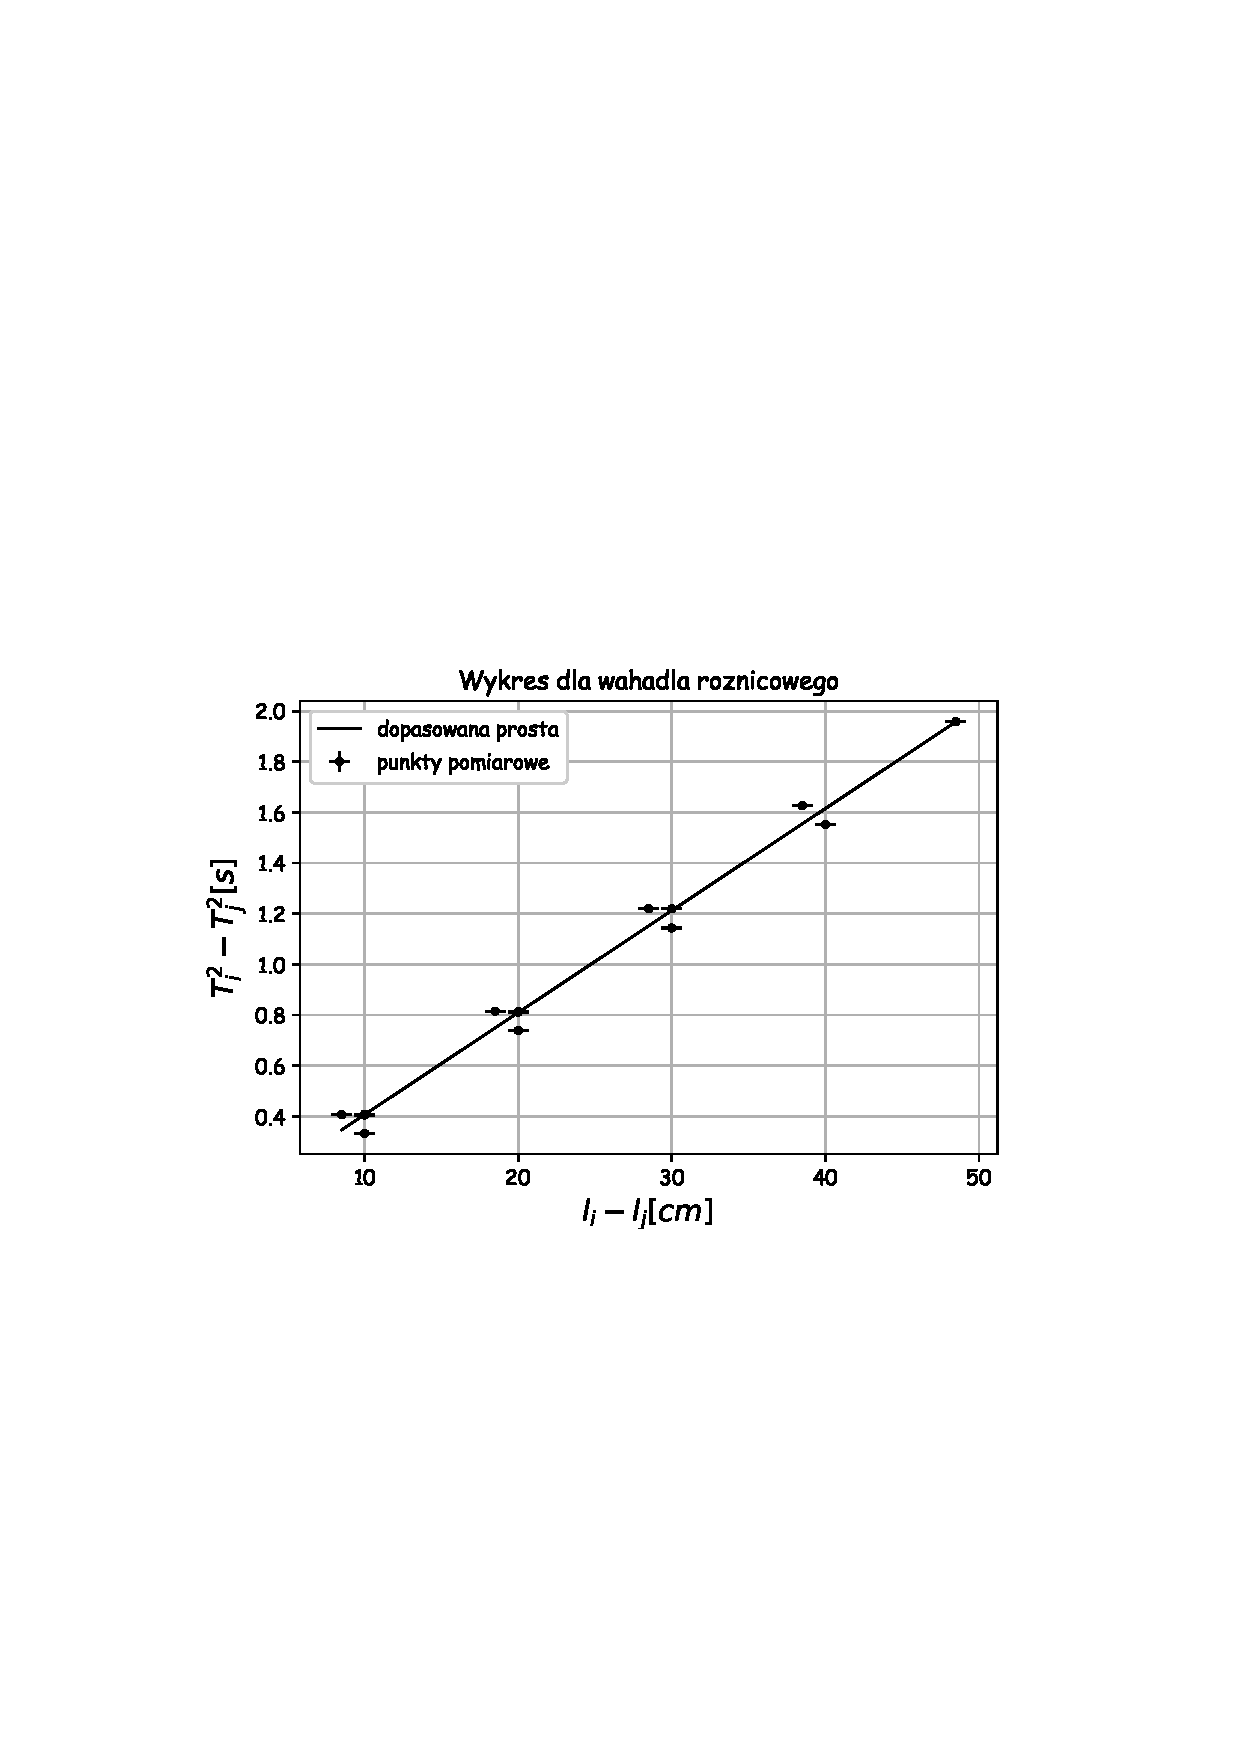
\includegraphics{./Wykres_roznicowe.png}
    \caption{}
    \label{}
\end{figure}

Wyliczona wartość przyspieszenia ziemskiego wynosi g = 9.841(0.299)[$\frac{m}{s^2}$]
\section{Analiza niepewności}

\section{Wnioski}


\end{document}
